\chapter{Outlier Detection based on Water level Data}
Create a connection between the theoretical descriptions of outlier detections to a real world use case. Data from \url{https://pegelalarm.at/}
\section{What is the Goal?}
Describe the goal to archive: \newline
\begin{itshape}
    ``
    \begin{enumerate}
        \item We are looking for an algorithm that detects outliers using only historical values. This would allow us to assign a probability to the last measured water level of a station, which would indicate how likely it is to be an outlier. We would then not store outliers in our system at all or classify them as outliers from the beginning.
        \item For us also an algorithm would be helpful, which assigns an outlier probability to each arbitrary measured value X of a time series. This algorithm would not only have access to the measured values before it, but also to those after it. This would allow us to detect outliers for all the time series data that we already have in the system and, for example, delete them.

    \end{enumerate}
    Point 2 is probably easier to implement than point 1, so an algorithm 1 would be more helpful for us.
    Also important would be that the algorithm adjusts its (hyper)parameters accordingly based on the historical data. This means that a level at which there are often strong fluctuations, an outlier must already be quite outlier so that it is considered as an outlier.
    ''
\end{itshape}

\section{How to retrieve the Data (Description of the API)}
Short overview on how to use the API to retrieve data? Python project to retrieve data: \url{https://github.com/SOBOS-GmbH/pegelalarm_public_pas_doc}
\section{Overview of the Data}
Provide an overview oth the data.
\section{Explorative Data Analysis}
Similar to overview of the data
\section{Manually detect outliers for a subset of data}
Show cases of outliers in the data and manually classify them. (Also define a way/data structure to classify outliers for time series data)
\newline
\newline
In order to speed up the manual labeling of outliers a program was written. The program is a Plotly \todo{add reference} Dash web application which displays the water level data as a scatter chart. 
By clicking the datapoints in the chart the user is able to toggle the datapoint as an outlier or back to a regular value. 
In Listing \ref{listing:manual-outlier-selection} the source code of the Dash application is shown. 
In \ref{figure:manual-outlier-selection} you can see the Website of the Python app. Below the chart a rangeslider is located, to move the zoomed in view horizontally. 
The refresh button on the left side refreshes the graph, thus updating the color and label of previously selected outliers. Furthermore it saves the data to a parquet file.
The upper and lower limit of the y-axis also gets updated, when pressing the refresh button. 
The limits are automatically set to the lowest and highest regular value. 
This was implemented, because some datasets had outliers with a huge difference towards the regular data. 
Without the automatic scaling of the y-axis, detecting other outliers with a smaller difference was not possible.
% \begin{center}
%     \makebox[\textwidth]{\includegraphics[width=\paperwidth]{...}}
%   \end{center}
\begin{figure}[H]
    \centering
    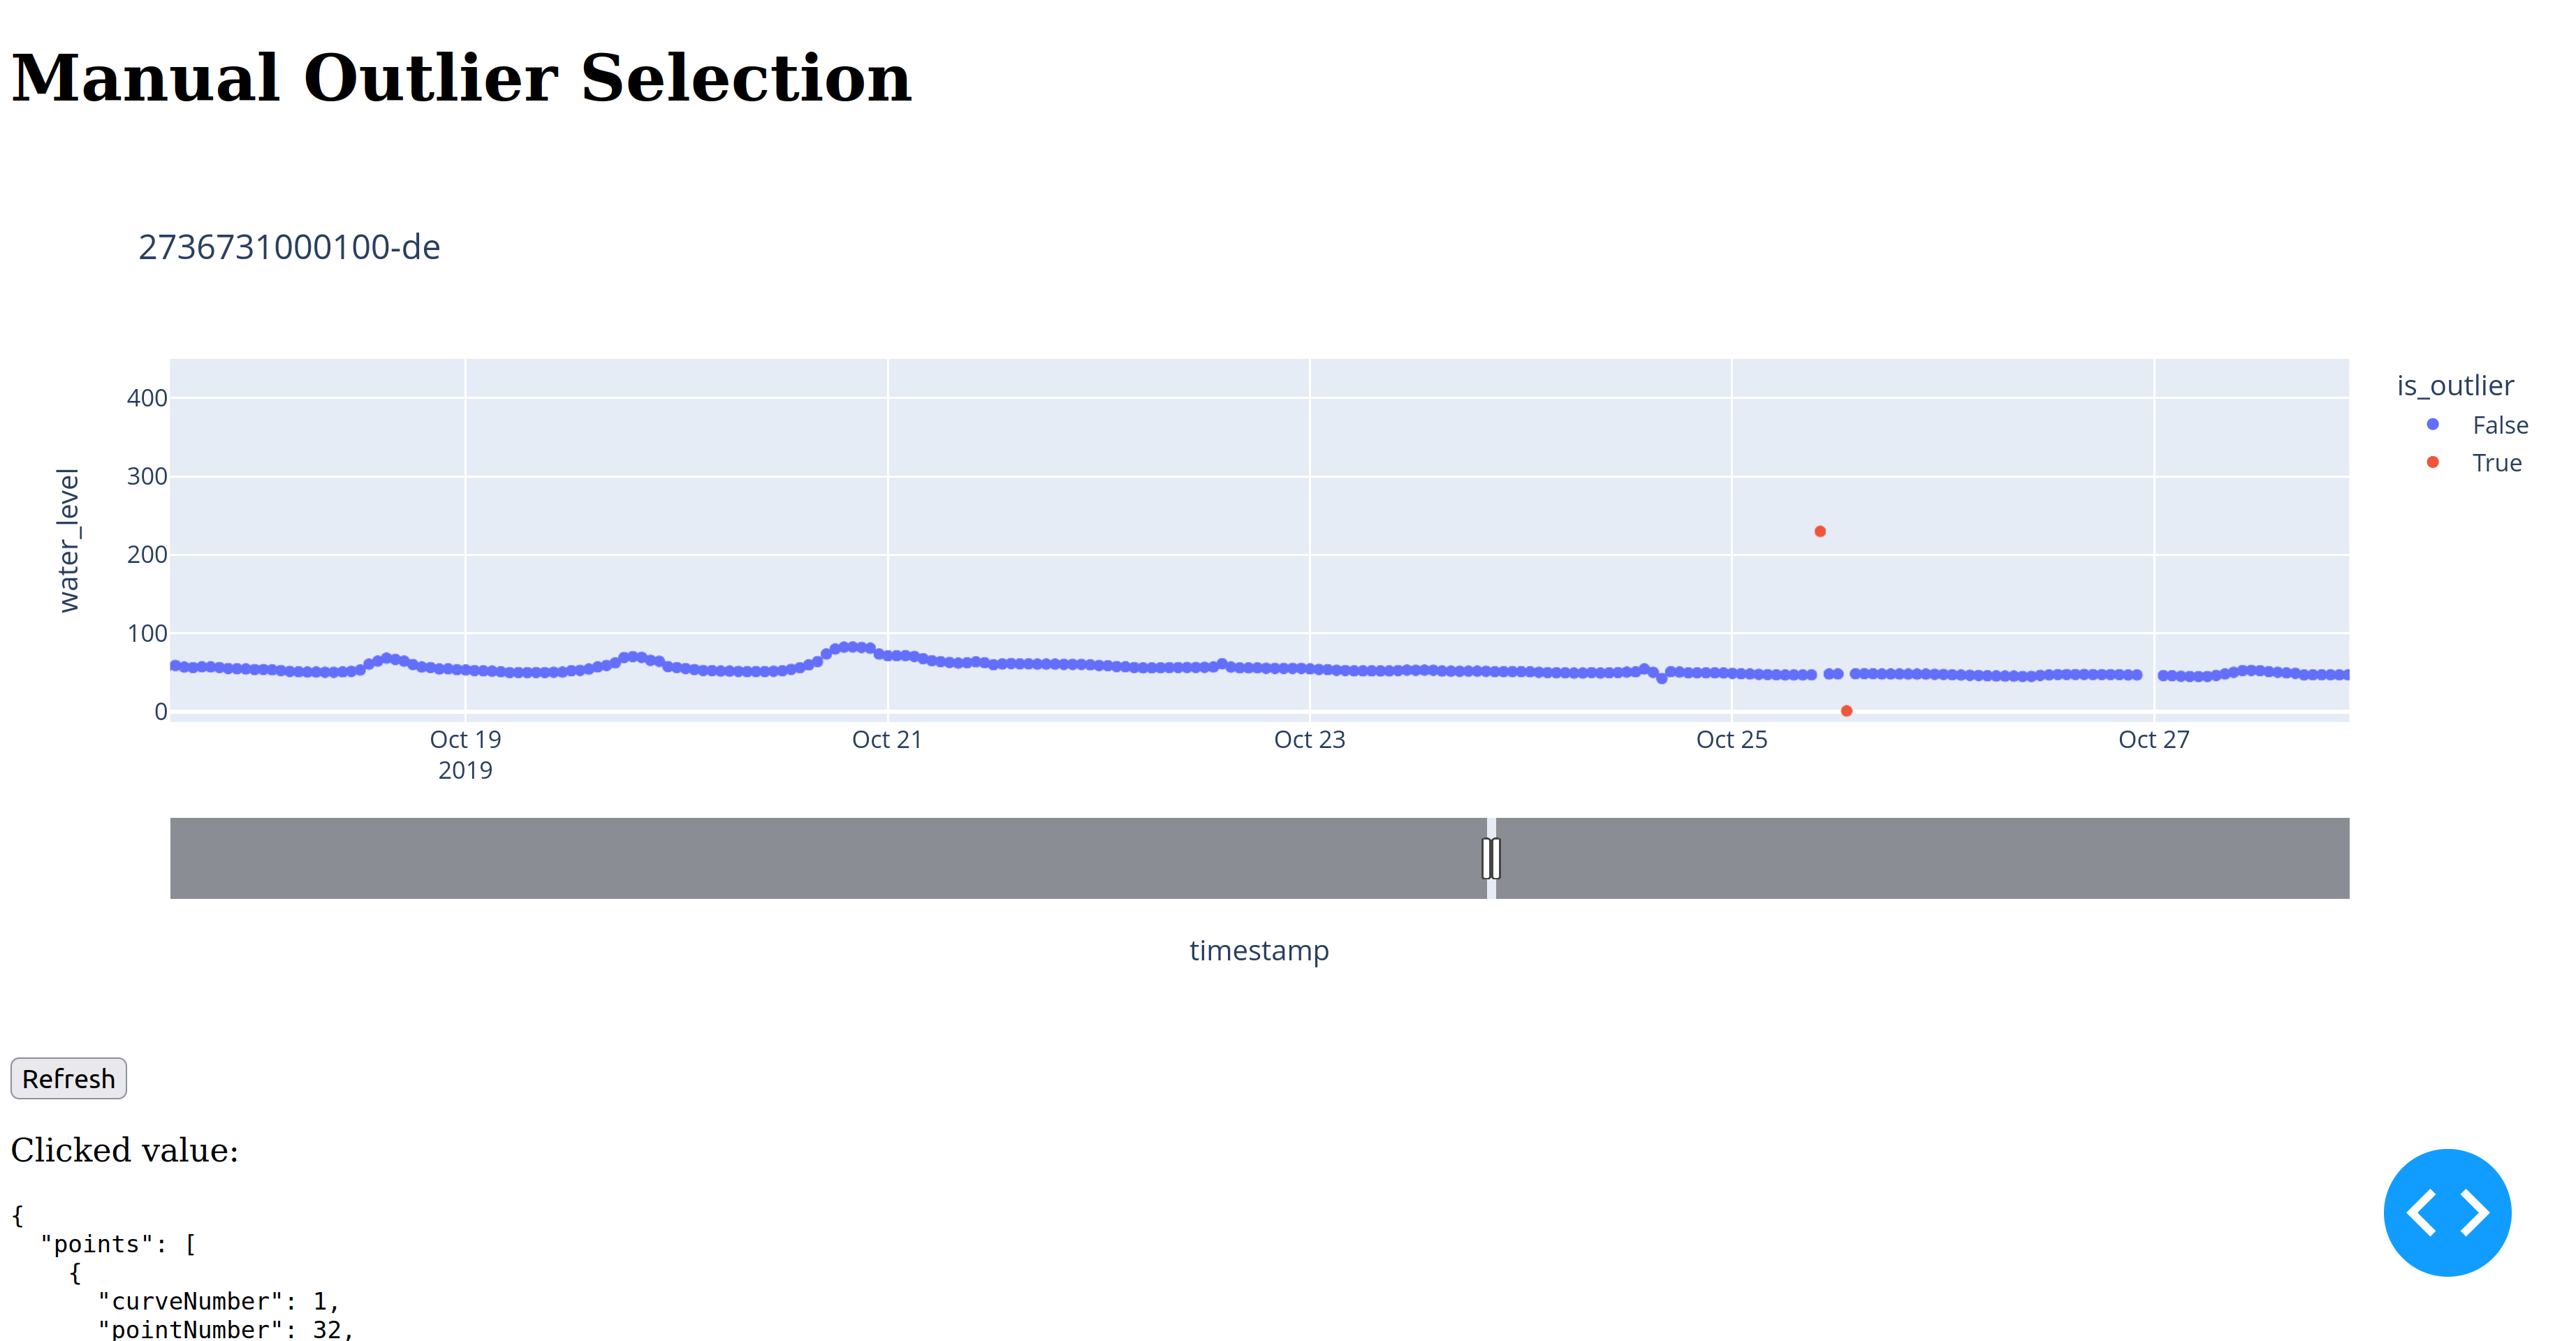
\includegraphics[width=\textwidth]{./pics/manual-outlier-selection.png}
    \caption{Dash Webapp to classify outliers}
    \label{figure:manual-outlier-selection}
\end{figure}

% https://tex.stackexchange.com/questions/368864/pagebreak-for-minted-in-figure
% \begin{listing}
% \begin{minted}[frame=single]{python}
% print('hw')
% \end{minted}
% \caption{Code example with simple formatting}
% \label{code:manual-outlier-selection}
% \end{listing}

\subsubsection{Manual Outlier Detection Webapp using Dash}
\inputminted[linenos]{python}{./code/manual_outlier_detection.py}
\captionof{listing}{Manual Outlier Detection Webapp using Dash\label{listing:manual-outlier-selection}}
\todo{add comments to code}

\section{Define Outlier Detection performance Metrics given on a Subset of Data}
Define a way to compare different outlier detection models / define performance metrics. E.g. number correct outliers, average confidence for the correct outliers, number of missed outliers,....
\section{Implement different Outlier Detection Approaches}
Develop different outlier detection methods in Python and calculate performance metrics for each
\section{Compare different Outlier Detection Approaches}
Compare detection methods from the previous section.

